\documentclass{beamer}
\usepackage[utf8]{inputenc}
\usepackage[T1]{fontenc}
\usepackage[ngerman]{babel}
\usepackage{times}
\usepackage{graphicx}
\usepackage{multirow}

\usetheme{Boadilla}

\title[DXRAM]{DXRAM\\Log + Recovery}

\author{Florian Klein}

\institute[Universität Düsseldorf] {Institut für Informatik\\Abteilung Betriebssysteme\\Heinrich-Heine-Universität Düsseldorf}

\date{11.12.2012}

\titlegraphic{
\includegraphics[width=3cm]{../img/hhulogo}}

\begin{document}

\section*{Title}

	\begin{frame}
		\titlepage
	\end{frame}

\section*{Outline}

	\begin{frame}
		\frametitle{Outline}

		\tableofcontents[hideallsubsections]
	\end{frame}

\section{Data-Structure}

	\begin{frame}
		\frametitle{Data-Structure}

		\begin{block}{ChunkInformation}
			\begin{tabular}{|l|l|l|}
				\hline
				\emph{Field}		&\emph{Type}		&\emph{Description}			\\\hline
				\texttt{m\_chunkID}	&\texttt{ID}		&unique Chunk-Identifier		\\\hline
				\texttt{m\_version}	&\texttt{long}		&version of the Chunk			\\\hline
				\texttt{m\_flags}	&\texttt{int}		&flags (present, foreign)		\\\hline
				\texttt{m\_nodeID}	&\texttt{NodeID}	&unique identifier of the hosting Node	\\\hline
			\end{tabular}
		\end{block}

		\begin{block}{Chunk extends ChunkInformation}
			\begin{tabular}{|l|l|l|}
				\hline
				\emph{Field}		&\emph{Type}		&\emph{Description}	\\\hline
				\texttt{m\_data}	&\texttt{ByteBuffer}	&binary data		\\\hline
			\end{tabular}
		\end{block}
	\end{frame}

\section{Log}

	\begin{frame}
		\frametitle{Outline}

		\tableofcontents[currentsection, hideothersubsections]
	\end{frame}

\subsection{Current Log-Layout}

	\begin{frame}
		\frametitle{Types}

		\begin{block}{Block}
			\begin{itemize}
				\item stores a Chunk
				\item default 1 MB
			\end{itemize}
		\end{block}

		\begin{block}{Segment}
			\begin{itemize}
				\item merges a number of Chunks
				\item backup entity
				\item default 64 MB
			\end{itemize}
		\end{block}
	\end{frame}

	\begin{frame}
		\frametitle{Meta-Data I}

		\begin{block}{Segment-Header}
			\begin{itemize}
				\item Segment-Index (4 Byte)
				\item Flags (4 Byte)
					\begin{itemize}
						\item empty
						\item full
						\item foreign
						\item number of free Blocks
					\end{itemize}
				\item Bitmap (1 Bit per Block in the Segment)
			\end{itemize}
		\end{block}

		\begin{exampleblock}{Bitmap (64 MB Segments and 1 MB Blocks)}
			$\Rightarrow$ 64 Blocks per Segment
			$\Rightarrow$ 8 Byte Bitmap
		\end{exampleblock}

		\begin{exampleblock}{Bitmap (64 MB Segments and 1 KB Blocks)}
			$\Rightarrow$ 65536 Blocks per Segment
			$\Rightarrow$ 8192 Byte Bitmap
		\end{exampleblock}
	\end{frame}

	\begin{frame}
		\frametitle{Meta-Data II}

		\begin{block}{Log-Header}
			Hash-Table with one entry per Block
			\begin{tabular}{|r|l|l|l|}
				\hline
				\emph{Bytes}	&\emph{Content}	&\multicolumn{2}{|c|}{\emph{Type}}							\\\hline
				1		&valid-flag	&\multicolumn{2}{|c|}{\texttt{boolean}}							\\\hline
				4		&ID length	&\multirow{2}{*}{\texttt{ID}}		&\multirow{7}{*}{\texttt{ChunkInformation}}	\\\cline{1-2}
				20		&ID bytes	&					&						\\\cline{1-3}
				8		&version	&\texttt{long}				&						\\\cline{1-3}
				4		&flags		&\texttt{int}				&						\\\cline{1-3}
				4		&host length	&\multirow{3}{*}{\texttt{NodeID}}	&						\\\cline{1-2}
				15		&host		&					&						\\\cline{1-2}
				2		&port		&					&						\\\hline
				8		&address	&\texttt{long}				&\multirow{2}{*}{\texttt{StorageInformation}}	\\\cline{1-3}
				4		&size		&\texttt{int}				&						\\\hline\cline{1-1}
				70		&\multicolumn{3}{c}{}											\\\cline{1-1}
			\end{tabular}
		\end{block}
	\end{frame}

	\begin{frame}
		\frametitle{Layout}

		\begin{block}{Initial situation}
			\center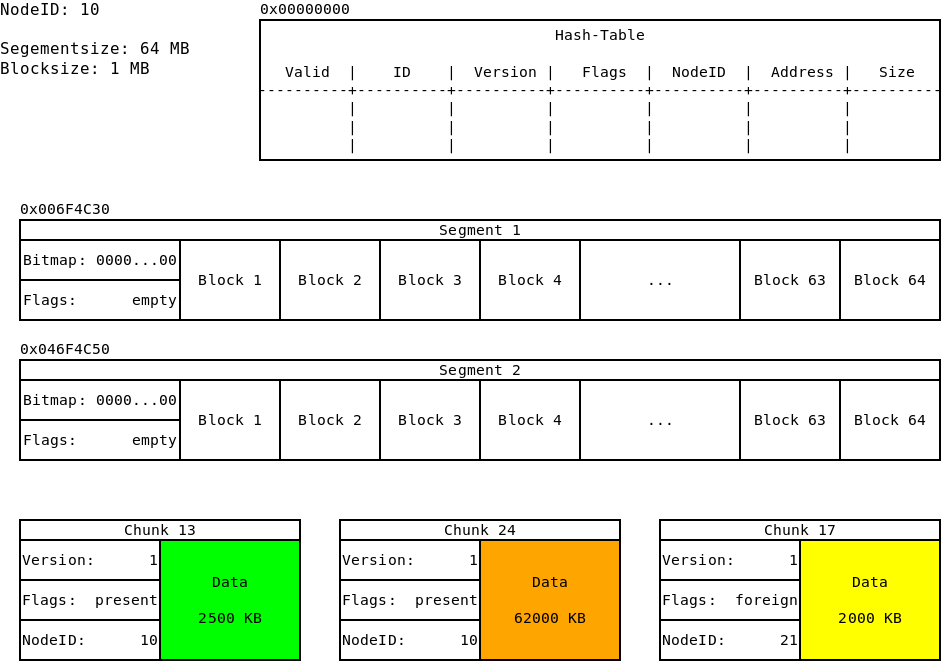
\includegraphics[width=9cm]{./img/Log_Layout_00}
		\end{block}
	\end{frame}

	\begin{frame}
		\frametitle{Layout}

		\begin{block}{Inserting Chunk 13}
			\center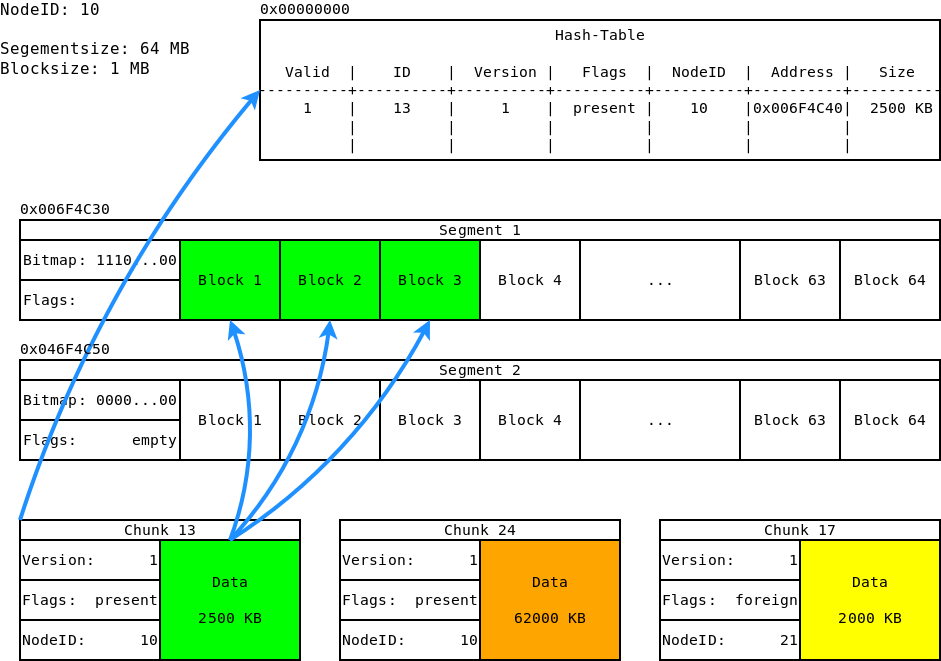
\includegraphics[width=9cm]{./img/Log_Layout_01}
		\end{block}
	\end{frame}

	\begin{frame}
		\frametitle{Layout}

		\begin{block}{Inserting Chunk 24}
			\center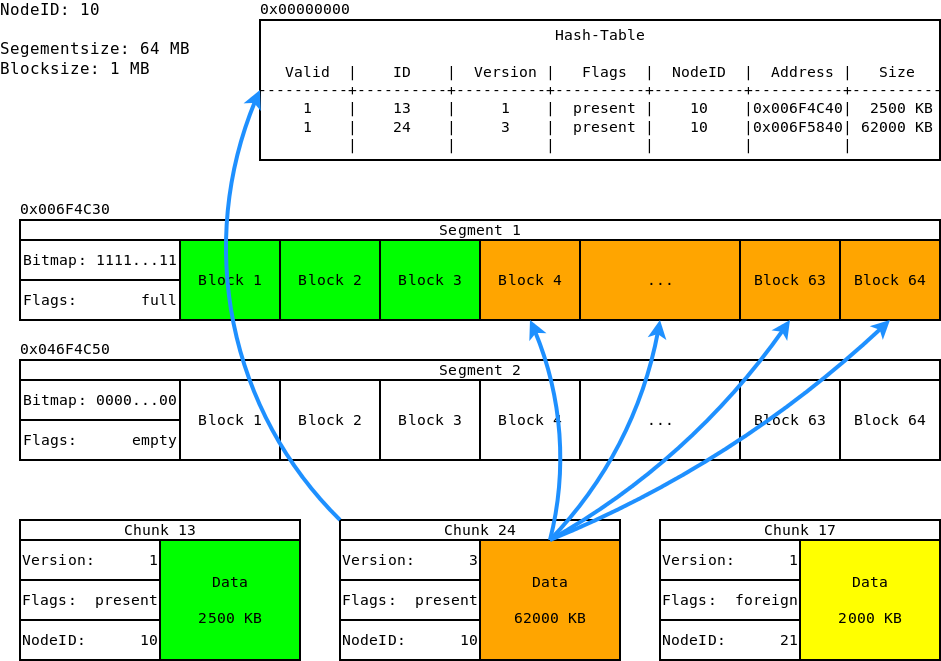
\includegraphics[width=9cm]{./img/Log_Layout_02}
		\end{block}
	\end{frame}

	\begin{frame}
		\frametitle{Layout}

		\begin{block}{Inserting Chunk 17}
			\center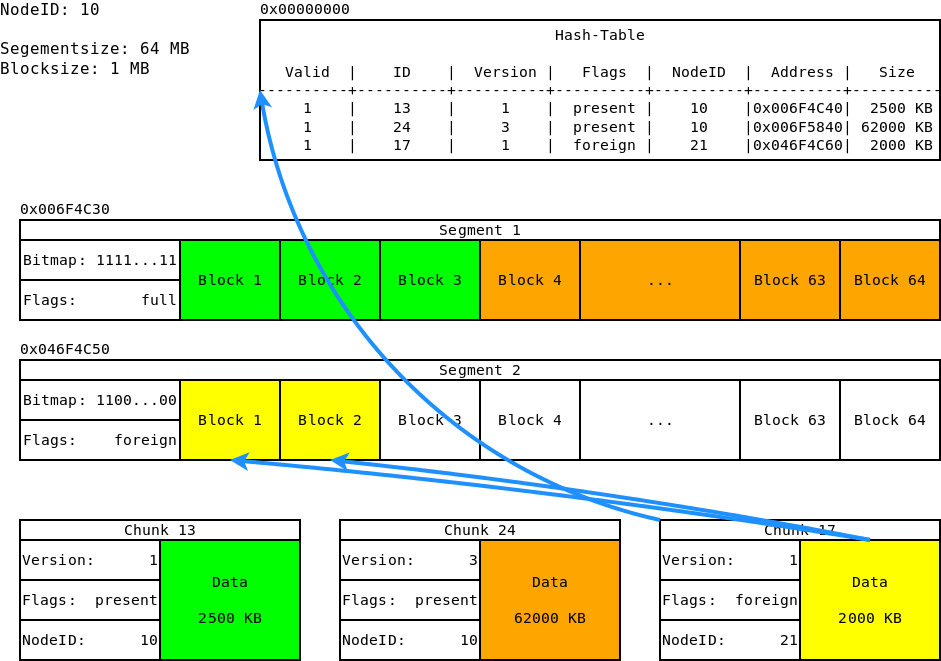
\includegraphics[width=9cm]{./img/Log_Layout_03}
		\end{block}
	\end{frame}

	\begin{frame}
		\frametitle{Layout}

		\begin{block}{Final situation}
			\center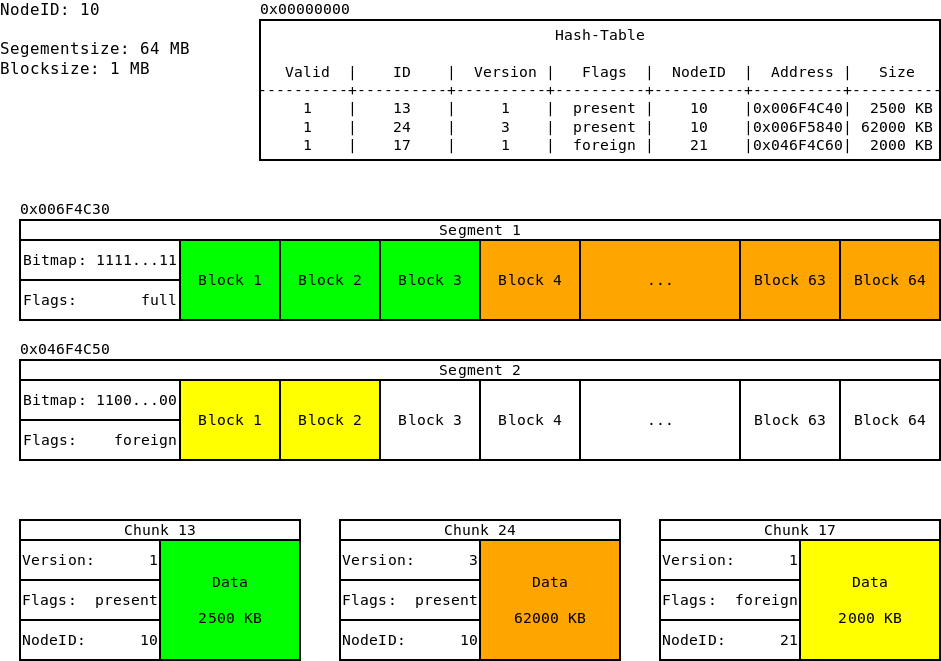
\includegraphics[width=9cm]{./img/Log_Layout_04}
		\end{block}
	\end{frame}

	\begin{frame}
		\frametitle{Overhead}

		\begin{block}{Log-Header}
			\begin{itemize}
				\item 70 Bytes per Block
			\end{itemize}
		\end{block}

		\begin{block}{Segment-Header}
			\begin{itemize}
				\item 1 Bit per Block
				\item 8 Bytes per Segment
			\end{itemize}
		\end{block}
	\end{frame}

	\begin{frame}
		\frametitle{Overhead examples}

		\begin{exampleblock}{100 GB Log-File, 64 MB Segments and 1 MB Blocks}
			$\Rightarrow$ 1.600 Segements each with 64 Blocks\\
			$\Rightarrow$ 102.400 Blocks\\
			\vspace{0.3cm}
			$1.600 * 8 B + 102.400 * 1 Bit + 102.400 * 70 B$\\
			$= 12.800 B + 12.800 B + 7.168.000 B = 7.193.600 B$\\
			$\approx 7 MB$
		\end{exampleblock}

		\begin{exampleblock}{100 GB Log-File, 64 MB Segments and 1 KB Blocks}
			$\Rightarrow$ 1.600 Segements each with 65536 Blocks\\
			$\Rightarrow$ 104.857.600 Blocks\\
			\vspace{0.3cm}
			$1.600 * 8 B + 104.857.600 * 1 Bit + 104.857.600 * 70 B$\\
			$= 12.800 B + 13.107.200 B + 7.340.032.000 B = 7.353.152.000 B$
			$\approx 7 GB$
		\end{exampleblock}
	\end{frame}

\subsection{Update process}

	\begin{frame}
		\frametitle{Update process (Overview)}

		\begin{block}{Initial situation}
			\center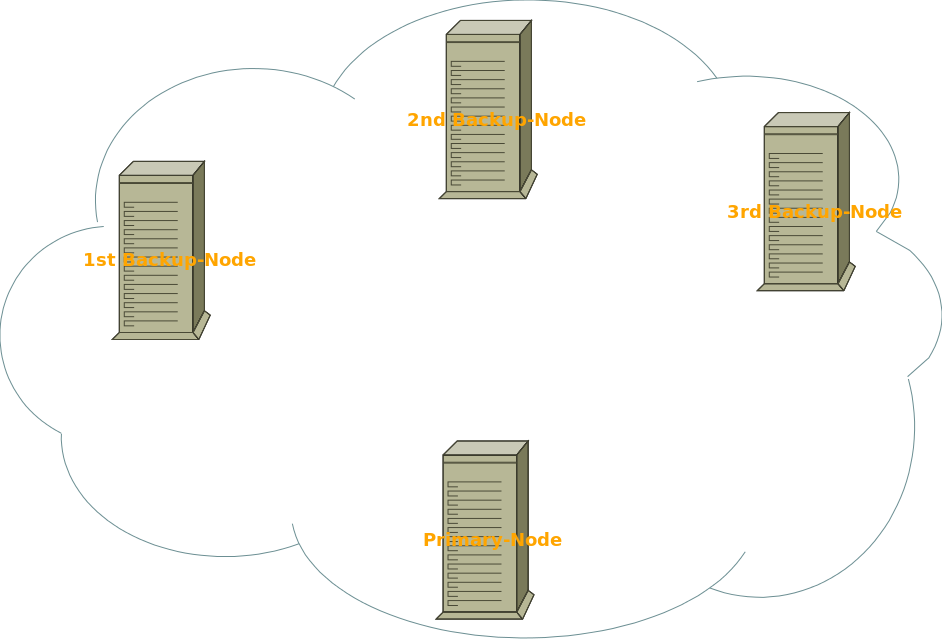
\includegraphics[width=8cm]{./img/Log_Overview_00}
		\end{block}
	\end{frame}

	\begin{frame}
		\frametitle{Update process (Overview)}

		\begin{block}{1. Step}
			\center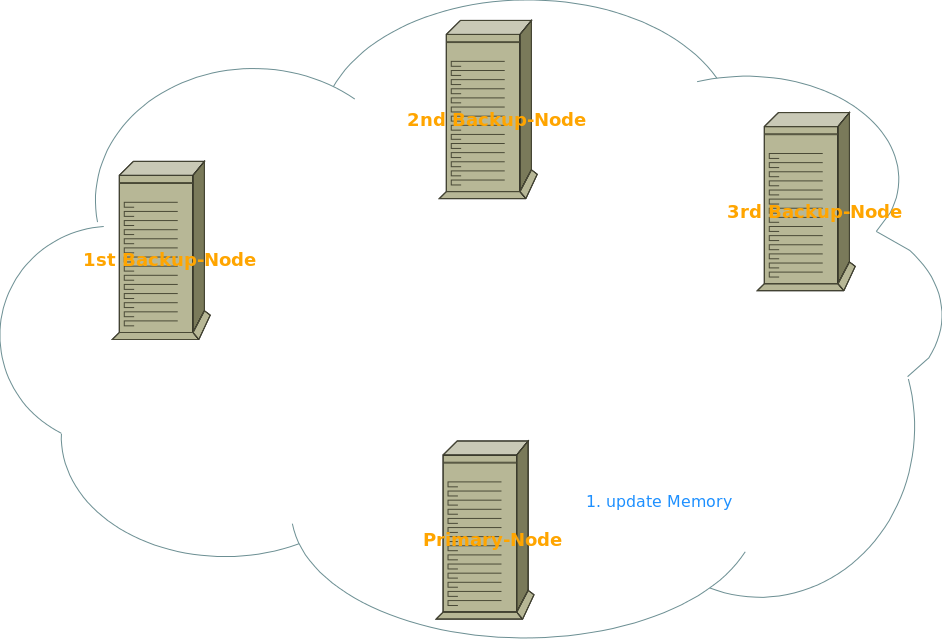
\includegraphics[width=8cm]{./img/Log_Overview_01}
		\end{block}
	\end{frame}

	\begin{frame}
		\frametitle{Update process (Overview)}

		\begin{block}{2. Step}
			\center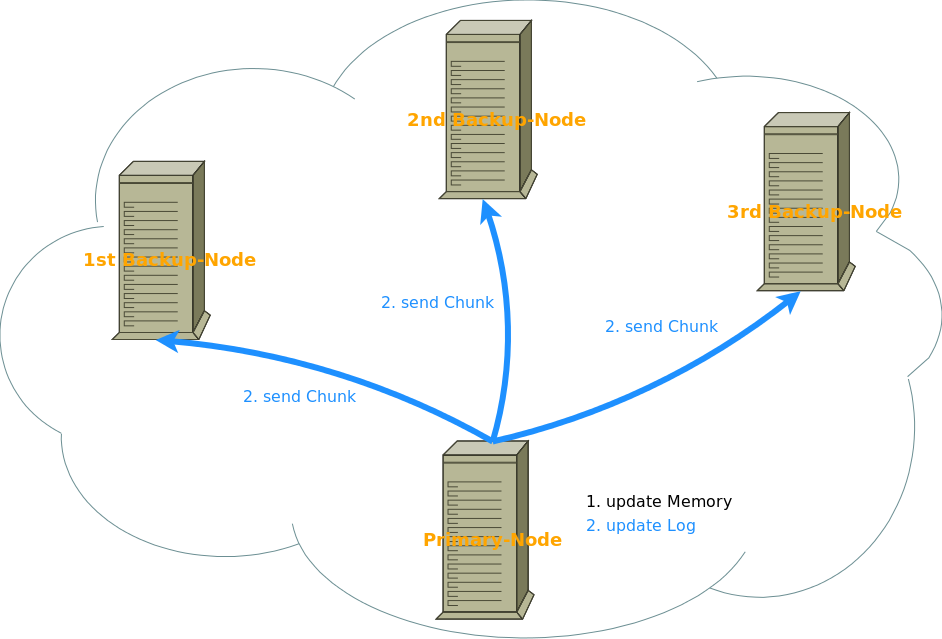
\includegraphics[width=8cm]{./img/Log_Overview_02}
		\end{block}
	\end{frame}

	\begin{frame}
		\frametitle{Update process (Overview)}

		\begin{block}{3. Step}
			\center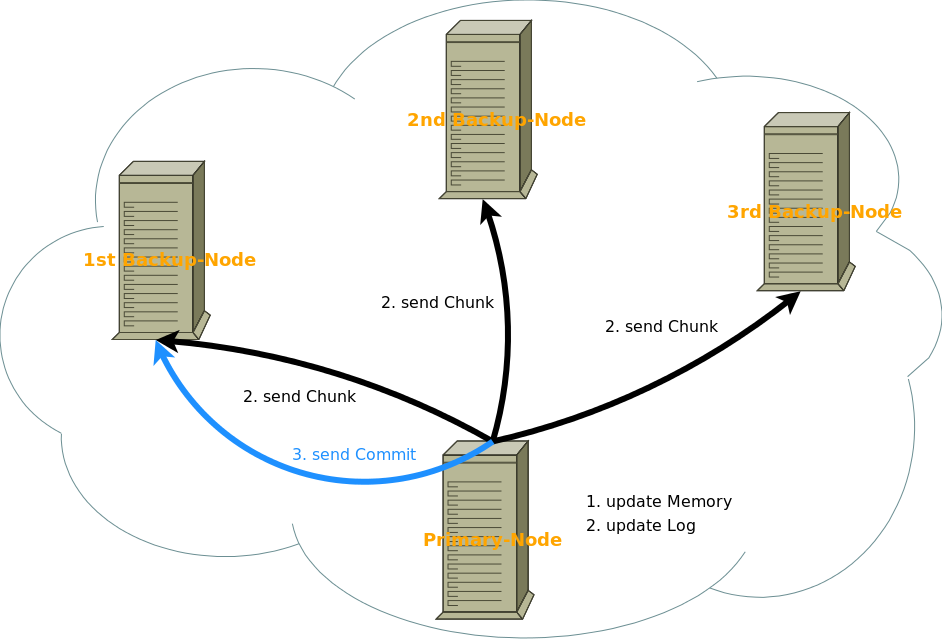
\includegraphics[width=8cm]{./img/Log_Overview_03}
		\end{block}
	\end{frame}

	\begin{frame}
		\frametitle{Update process (Overview)}

		\begin{block}{4. Step}
			\center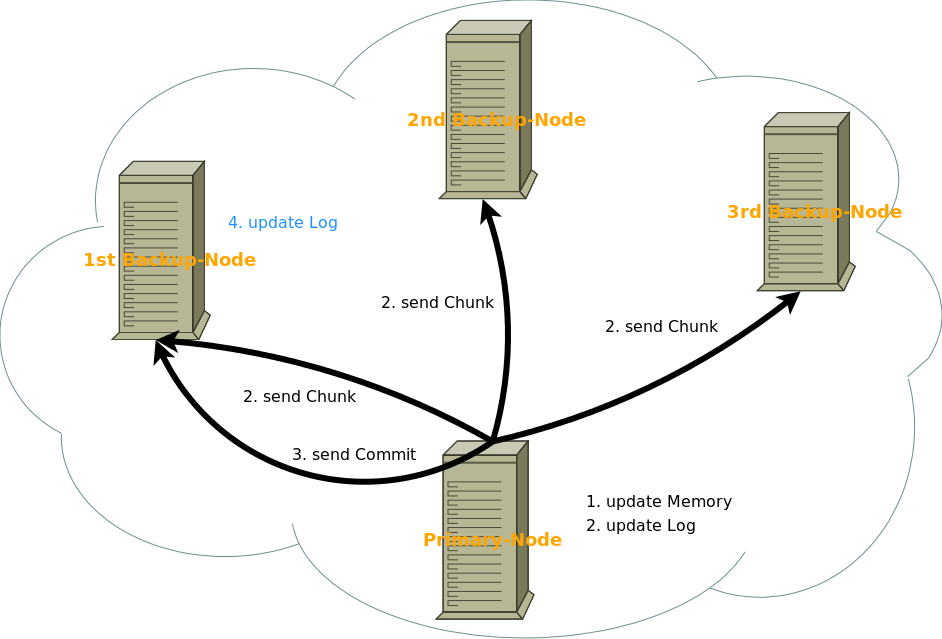
\includegraphics[width=8cm]{./img/Log_Overview_04}
		\end{block}
	\end{frame}

	\begin{frame}
		\frametitle{Update process (Overview)}

		\begin{block}{5. Step}
			\center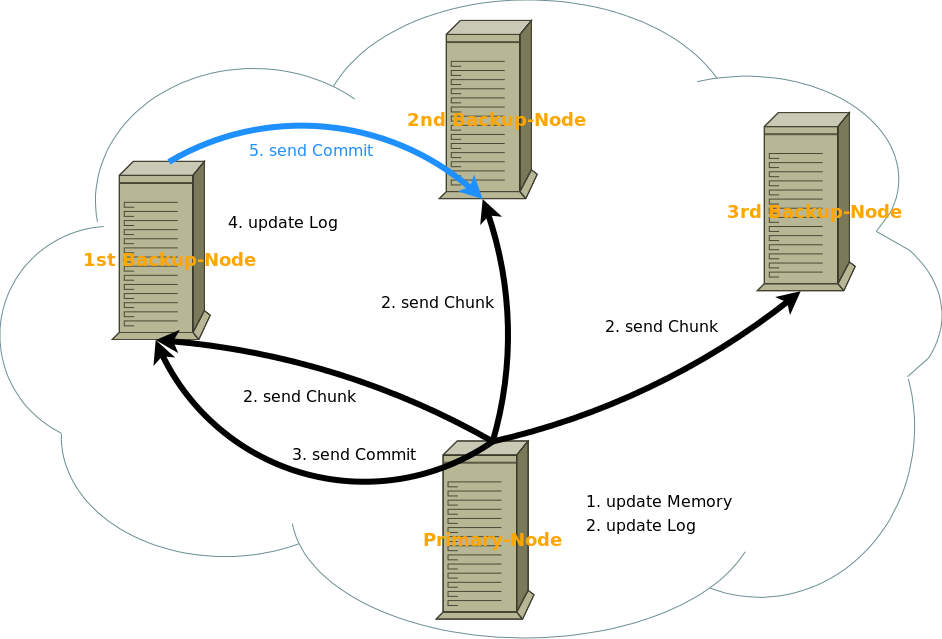
\includegraphics[width=8cm]{./img/Log_Overview_05}
		\end{block}
	\end{frame}

	\begin{frame}
		\frametitle{Update process (Overview)}

		\begin{block}{6. Step}
			\center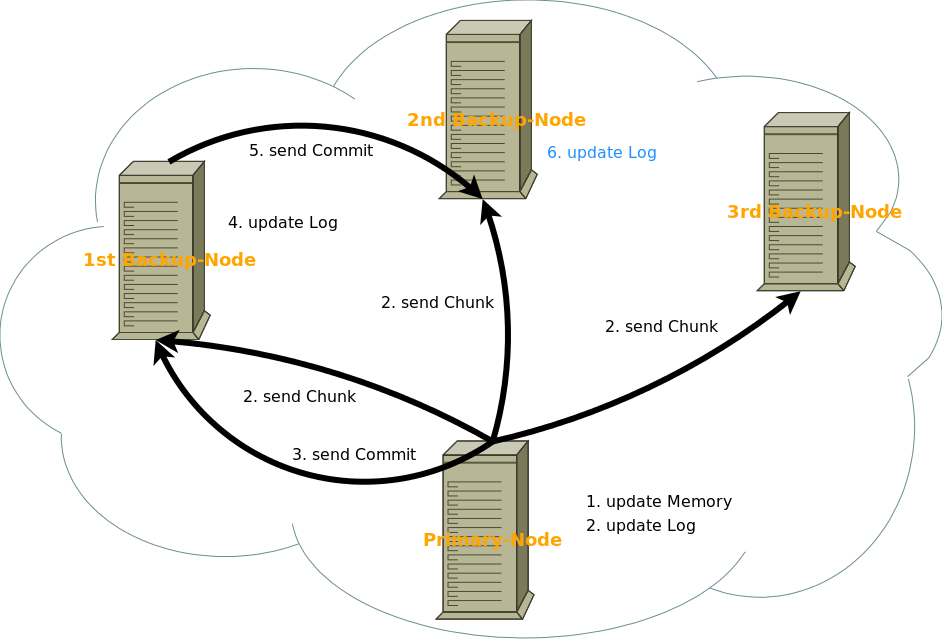
\includegraphics[width=8cm]{./img/Log_Overview_06}
		\end{block}
	\end{frame}

	\begin{frame}
		\frametitle{Update process (Overview)}

		\begin{block}{7. Step}
			\center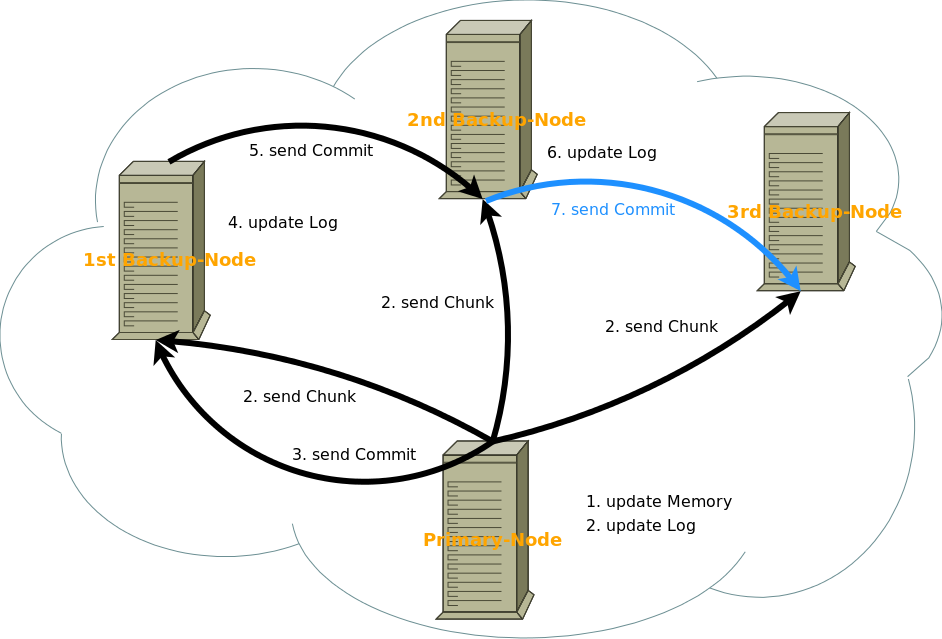
\includegraphics[width=8cm]{./img/Log_Overview_07}
		\end{block}
	\end{frame}

	\begin{frame}
		\frametitle{Update process (Overview)}

		\begin{block}{8. Step}
			\center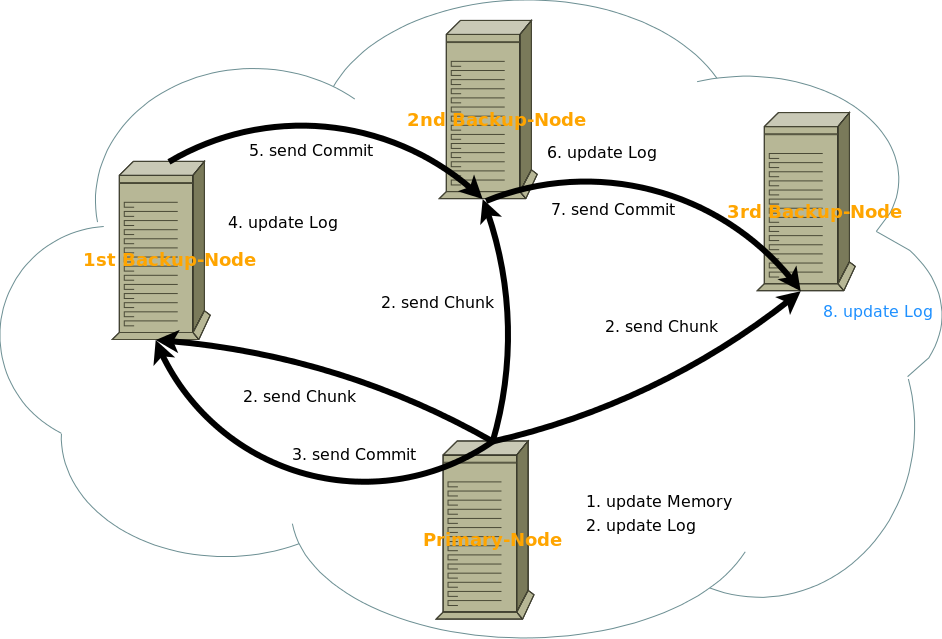
\includegraphics[width=8cm]{./img/Log_Overview_08}
		\end{block}
	\end{frame}

	\begin{frame}
		\frametitle{Update process (Overview)}

		\begin{block}{9. Step}
			\center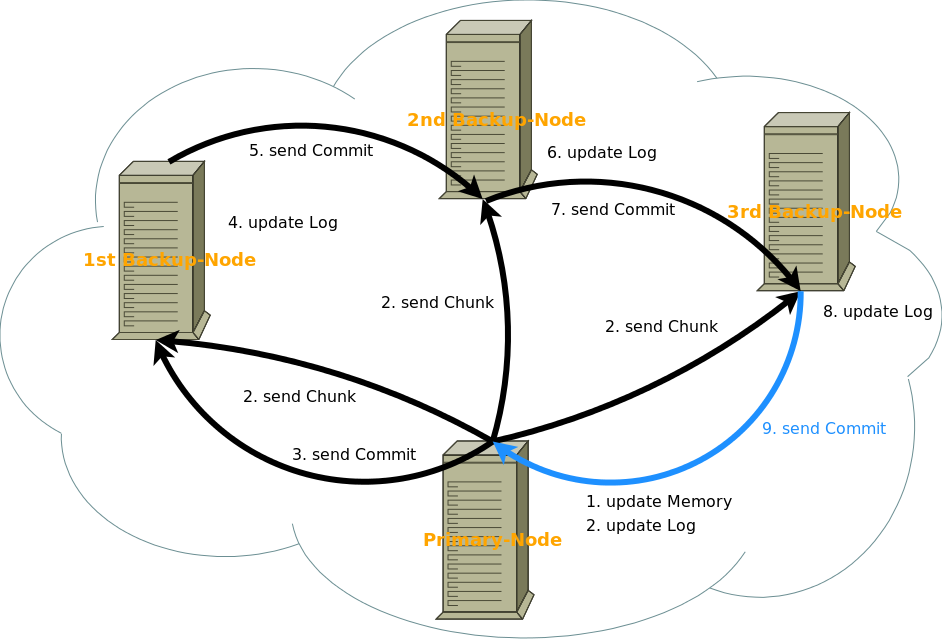
\includegraphics[width=8cm]{./img/Log_Overview_09}
		\end{block}
	\end{frame}

	\begin{frame}
		\frametitle{Update process (Overview)}

		\begin{block}{10. Step}
			\center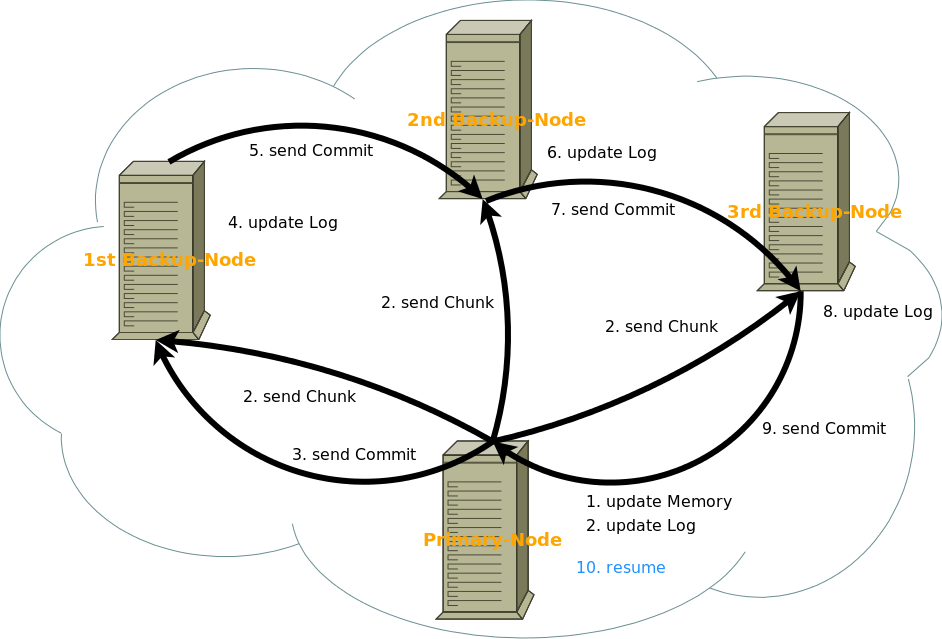
\includegraphics[width=8cm]{./img/Log_Overview_10}
		\end{block}
	\end{frame}

	\begin{frame}
		\frametitle{Update process I}

		\begin{block}{Memory (Primary-Node)}
			\begin{enumerate}[(a)]
				\item set dirty-bit
				\item update chunk in-place
				\item increment version
				\item clear dirty-bit
			\end{enumerate}
		\end{block}

		\begin{block}{Log (Primary-Node)}
			\begin{enumerate}[(a)]
				\item send chunk to the backup nodes
				\item update chunk
					\begin{description}
						\item[Solution 1:] in-place
						\item[Solution 2:] copy-on-write (RAMCloud)
						\item[Solution 3:] twins
					\end{description}
				\item send Commit-Message to $1^{st}$ Backup-Node
				\item wait for Commit-Message from $3^{rd}$ Backup-Node
			\end{enumerate}
		\end{block}
	\end{frame}

	\begin{frame}
		\frametitle{Update process II}

		\begin{block}{Log (Backup-Node)}
			\begin{enumerate}[(a)]
				\item receive chunk from Primary-Node
				\item buffer chunk
				\item wait for Commit-Message from predecessor
				\item update chunk (like Primary-Node)
				\item send Commit-Message to successor
			\end{enumerate}
		\end{block}

		\begin{alertblock}{Problems}
			\begin{itemize}
				\item Primary-Node crashes before sending the Commit-Message
				\item Backup-Node crashes
			\end{itemize}
		\end{alertblock}
	\end{frame}

\section{Recovery}

	\begin{frame}
		\frametitle{Outline}

		\tableofcontents[currentsection, hideothersubsections]
	\end{frame}

\subsection{Peers and Super-Peers}

	\begin{frame}
		\frametitle{Super-Peer Overlay}

		\begin{block}{Overview}
			\center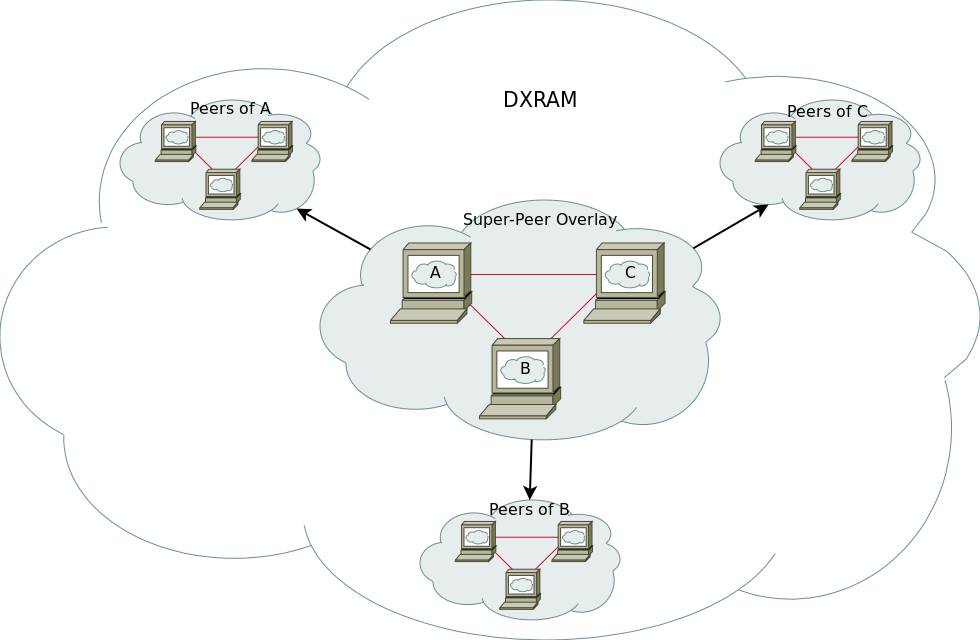
\includegraphics[width=10cm]{./img/Super-Peer_Overlay}
		\end{block}
	\end{frame}

	\begin{frame}
		\frametitle{Tasks}

		\begin{block}{Peer}
			\begin{itemize}
				\item stores Chunks in RAM
				\item logs own Chunks on SSD
				\item backups Chunks of other nodes on SSD
			\end{itemize}
		\end{block}

		\begin{block}{Super-Peer}
			\begin{itemize}
				\item also a Peer
				\item monitors its Peers (Heart-Beat)
				\item handles Meta-Data of Chunks (DHT-Node)
			\end{itemize}
		\end{block}
	\end{frame}

\subsection{Recovery process}

	\begin{frame}
		\frametitle{Recovery process (Overview)}

		\begin{block}{Initial situation}
			\center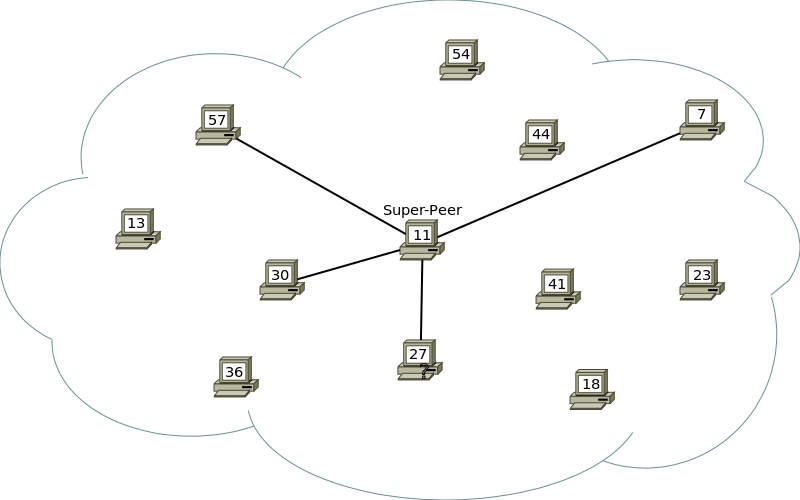
\includegraphics[width=8cm]{./img/Recovery_Overview_00}

			\begin{itemize}
				\item Super-Peer is connected with its Peers
			\end{itemize}
		\end{block}
	\end{frame}

	\begin{frame}
		\frametitle{Recovery process (Overview)}

		\begin{block}{Node failure}
			\center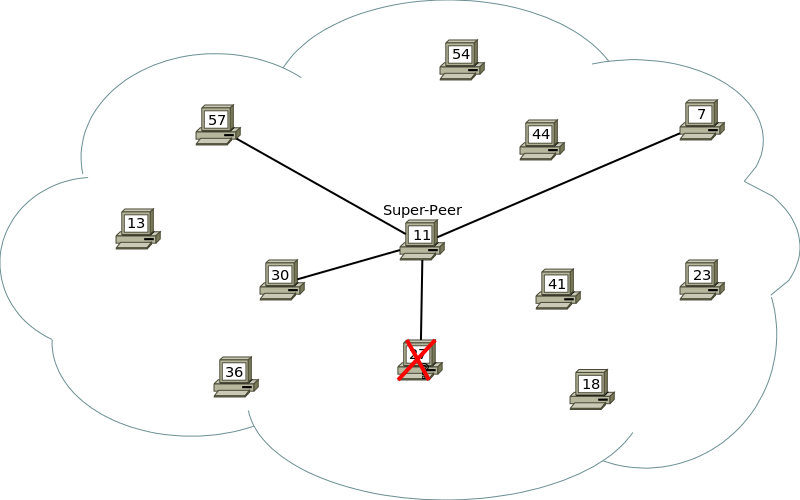
\includegraphics[width=8cm]{./img/Recovery_Overview_01}

			\begin{itemize}
				\item Node 27 crashes
			\end{itemize}
		\end{block}
	\end{frame}

	\begin{frame}
		\frametitle{Recovery process (Overview)}

		\begin{block}{Broadcast}
			\center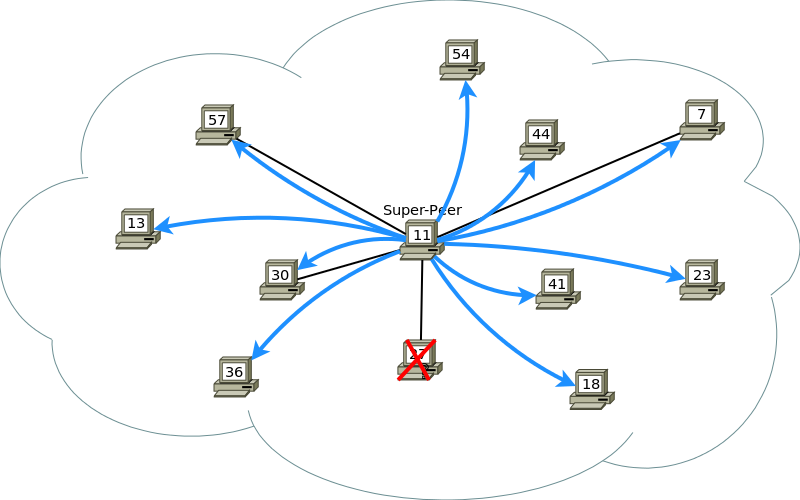
\includegraphics[width=8cm]{./img/Recovery_Overview_02}

			\begin{itemize}
				\item Super-Peer detects and broadcasts node failure
				\item Super-Peer becomes the Recovery Coordinator
			\end{itemize}
		\end{block}
	\end{frame}

	\begin{frame}
		\frametitle{Recovery process (Overview)}

		\begin{block}{Info-Message}
			\center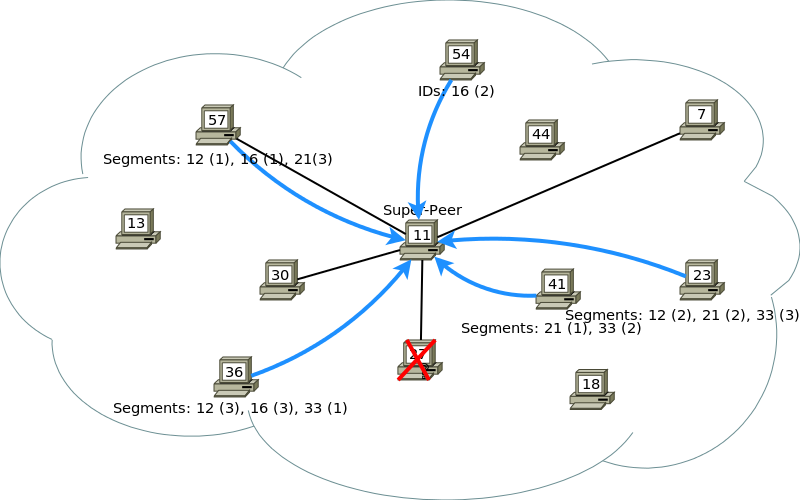
\includegraphics[width=8cm]{./img/Recovery_Overview_03}

			\begin{itemize}
				\item every node deletes cached Meta-Data of the failed node
				\item every Backup-Node of the failed node sends information about the backuped data to the Recovery Coordinator
				\item Recovery Coorinator gathers this information
			\end{itemize}
		\end{block}
	\end{frame}

	\begin{frame}
		\frametitle{Recovery process (Overview)}

		\begin{block}{Chunk recovery}
			\center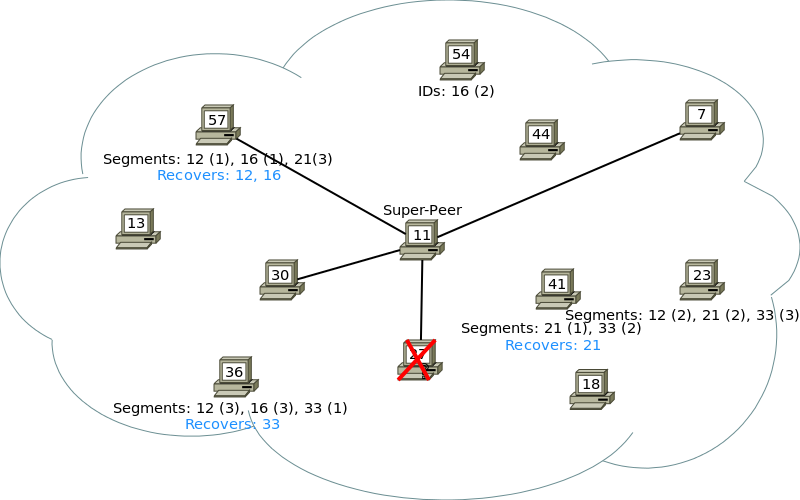
\includegraphics[width=8cm]{./img/Recovery_Overview_04}

			\begin{itemize}
				\item the $1^{st}$ Backup-Node of each segment recovers the segment
			\end{itemize}
		\end{block}
	\end{frame}

	\begin{frame}
		\frametitle{Recovery process (Overview)}

		\begin{block}{Commit-Message}
			\center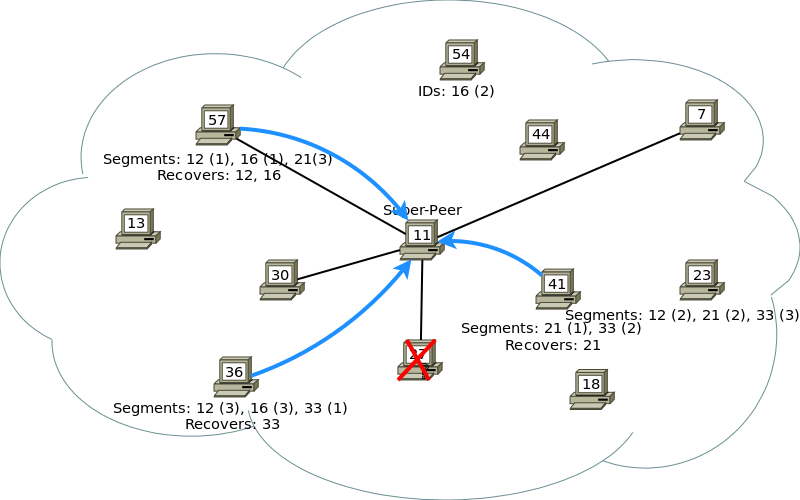
\includegraphics[width=8cm]{./img/Recovery_Overview_05}

			\begin{itemize}
				\item the $1^{st}$ Backup-Node of each segment send the result to the Recovery Coordinator
			\end{itemize}
		\end{block}
	\end{frame}

	\begin{frame}
		\frametitle{Recovery process (Overview)}

		\begin{block}{Final situation}
			\center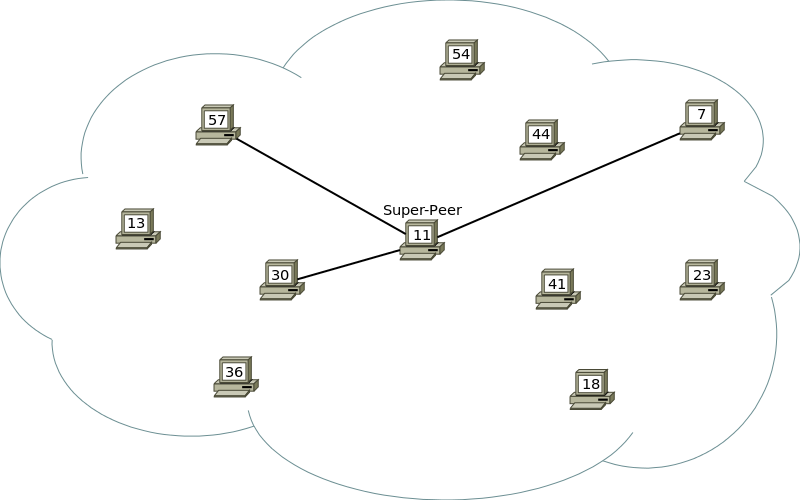
\includegraphics[width=8cm]{./img/Recovery_Overview_06}

			\begin{itemize}
				\item Recovery Coordinator updates Meta-Data for the recovered Segments/Chunks
				\item the failed node is removed
				\item an application callback can be executed (optional)
			\end{itemize}
		\end{block}
	\end{frame}

\section{Conclusion}

		\begin{frame}
			\frametitle{Conclusion}

			\begin{block}{Log}
				\begin{itemize}
					\item little overhead for objects $\ge 1 MB$ (e.g. Map \& Reduce)
					\item huge overhead for Objects $\le 1 KB$ (e.g. Facebook)
					\item[$\Rightarrow$] a new log layout have to be disigned for small objects
					\item the three update solutions must be compared
				\end{itemize}
			\end{block}

			\begin{block}{Recovery}
				\begin{itemize}
					\item distributed recovery dependent on segment distribution
						\begin{itemize}
							\item high distribution allows fast recovery
							\item low distribution preserves locality
						\end{itemize}
					\item ignores workload of the Backup-Nodes
					\item \textcolor{red}{Problem: Not all data could be locally recovered (IO failure or insufficent memory space)}
					\item \textcolor{red}{Problem: Realisation of the application callback}
				\end{itemize}
			\end{block}
		\end{frame}

\section*{Questions}

		\begin{frame}
			\begin{block}{}
				\center\Large{Questions?}
			\end{block}
		\end{frame}

\end{document}
